%  !TeX  root  =  user_guide.tex

\section{Plugin Interpolazione}\label{sec:interpol}

% when the revision of a section has been finalized, 
% comment out the following line:
% \updatedisclaimer

Il plugin di interpolazione permette di generare un TIN (Triangulated Irregular Network) 
o un'interpolazione IDW (Inverse Distance Weighting) a partire da un layer vettoriale di
punti: è molto semplice da usare grazie all'interfaccia grafica intuitiva mostrata 
in Figura \ref{fig:interpolation_dialog}.

Il plugin richiede l'impostazione dei seguenti parametri:
\begin{itemize}[label=--]
\item \textbf{Input}: permette di selezionare un layer vettoriale di punti tra quelli caricati in QGIS. 
È possibile utilizzare dati provenienti da più layer: selezionare i layer di interesse dal menu 
\selectstring{Vettori}{\dots} e cliccare su \button{Aggiungi} per aggiungerli nel riquadro sottostante.
Nota: è possibile utilizzare linee e poligoni come vincoli per la triangolazione, specificando 
'Linee struttura' o 'Linee di interruzione' nel menu a discesa \dropmenuopt{Tipo}.
\item \textbf{Attributo interpolazione}: selezionare la colonna attributo contenente i valori 
da utilizzare per l'interpolazione o attivare la casella di controllo 
\checkbox{Usa la coordinata Z per l'interpolazione}.
\item \textbf{Metodo di interpolazione}: permette di selezionare il metodo di interpolazione, che può essere 
\selectstring{Metodo di interpolazione}{Interpolazione Triangolare (TIN)} o 
\selectstring{Metodo di interpolazione}{Distanza Inversa Ponderata (IDW)}.
\item \textbf{Numero di colonne}: numero di colonne del raster di output
\item \textbf{Numero di righe}: numero di righe del raster di output
\item \textbf{File di output}: nome del raster di output.
\end{itemize}

\begin{figure}[ht]
   \centering
   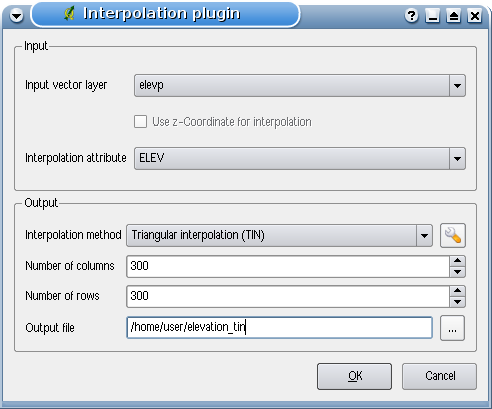
\includegraphics[clip=true, width=14cm]{interpolate_dialog}
   \caption{Plugin Interpolazione \nixcaption}\label{fig:interpolation_dialog}
\end{figure}

\minisec{Utilizzo del plugin}\label{interpolation_usage}

\begin{enumerate}
\item Avviare QGIS e caricare un layer vettoriale di punti (es. elevp.csv).  
  \item Caricare il plugin di Interpolazione nel gestore dei plugin (Sezione
  \ref{sec:load_core_plugin}) e cliccare su \toolbtntwo{interpolation}{Interpolazione} 
  nella barra dei plugin. La finestra di dialogo del plugin di Interpolazione appare 
  come in Figura \ref{fig:interpolation_dialog}.
  \item Selezionare \selectstring{elevp}{\ldots} come vettore di input e la colonna 
  \filename{ELEV} come attributo per interpolazione.
  \item Selezionare \selectstring{Interpolazione triangolare}{\ldots} come metodo di 
  interpolazione, impostare 5000 come dimensione delle celle e \filename{elevation\_tin} 
  come nome del raster di output.
  \item Cliccare su \button{Ok}.
  \item Aprire le proprietà di \filename{elevation\_tin} e selezionare \selectstring{Pseudocolor}{\ldots} come mappa di 
  colore nella scheda \tab{Stile}: e possibile definire una nuova mappa colore 
  come descritto nella Sezione \ref{label_rasterprop}.
\end{enumerate}

Nella Figura \ref{fig:interpolation_tin} si vede il risultato di una interpolazione TIN 
dei dati \filename{elevp.csv} visualizzati usando la mappa colore Pseudocolor. 
L'elaborazione richiede alcuni minuti.

\begin{figure}[ht]
   \centering
   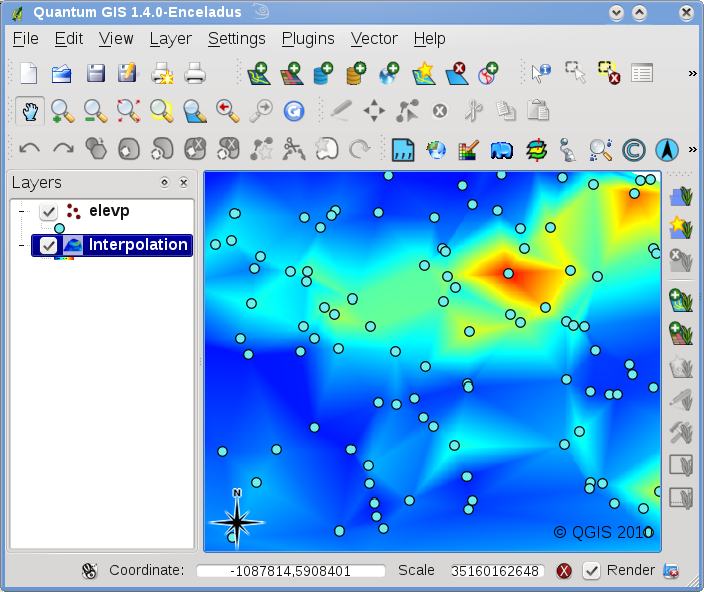
\includegraphics[clip=true, width=10cm]{interpolate_tin}
   \caption{Interpolazione dei dati elevp con metodo TIN \nixcaption}\label{fig:interpolation_tin}
\end{figure}

\FloatBarrier